\documentclass[11pt,a4paper]{article}

% ==================== PACKAGES ====================
\usepackage[utf8]{inputenc}
\usepackage[T1]{fontenc}
\usepackage{lmodern}
\usepackage{longtable}
\usepackage{array}
\usepackage{booktabs}
\usepackage{colortbl}
\usepackage{float}
\usepackage{xcolor}
\usepackage{titlesec}
\usepackage{fancyhdr}
\usepackage{enumitem}
\usepackage{hyperref}
\usepackage{parskip}
\usepackage[export]{adjustbox}
\usepackage{ragged2e}
\usepackage{graphicx}
\usepackage[margin=2.5cm]{geometry}

% ==================== COULEURS ====================
\definecolor{primaryblue}{RGB}{31,73,125}
\definecolor{lightgray}{RGB}{240,240,240}
\definecolor{tableheader}{RGB}{68,114,196}

% ==================== TITRES ====================
\renewcommand{\contentsname}{Table des matières}
\titleformat{\section}
  {\normalfont\Large\bfseries\color{primaryblue}}
  {\thesection}{1em}{}
\titleformat{\subsection}
  {\normalfont\large\bfseries\color{primaryblue}}
  {\thesubsection}{1em}{}

% ==================== EN-TETE / PIED DE PAGE ====================
\pagestyle{fancy}
\fancyhf{}
\fancyhead[L]{\small Document d'expression de besoins}
\fancyhead[R]{\small Gestion des flottes GSM / Fixe / ADSL / Fibre}
\fancyfoot[C]{\small\thepage}
\renewcommand{\headrulewidth}{0.4pt}

% ==================== HYPERLIENS ====================
\hypersetup{
  colorlinks=true,
  linkcolor=primaryblue,
  urlcolor=primaryblue,
  pdftitle={Document d'expression de besoins - Gestion des flottes télécoms},
  pdfauthor={A compléter}
}

% ==================== COMMANDES UTILES ====================
\newcolumntype{L}[1]{>{\RaggedRight\arraybackslash}p{#1}}

\newenvironment{infotable}
  {\begin{longtable}{L{4cm} L{11cm}}
   \toprule
   \rowcolor{tableheader}\textcolor{white}{\textbf{Élément}} & \textcolor{white}{\textbf{Détail}} \\
   \midrule
   \endhead}
  {\bottomrule\end{longtable}}

\title{\textbf{\Huge Document d'expression de besoins}\\[0.5em]
\Large Projet de gestion des flottes GSM / Fixe / ADSL / Fibre optique}
\author{}
\date{}

\begin{document}

\begin{titlepage}
\centering
\vspace*{2cm}
{\Huge\bfseries\color{primaryblue} Document d'expression de besoins\par}
\vspace{1cm}
{\Large Projet de gestion des flottes\par}
\vspace{1.5cm}
{\color{primaryblue}\rule{0.6\textwidth}{0.4pt}\par}
\vspace{1.5cm}
{\large\bfseries Wilaya de la Région Souss-Massa\\
Préfecture d'Agadir Ida Outanane\par}
\vspace{2cm}
{\normalsize Organisation publique\par}
\vspace{0.5cm}
{\normalsize \today\par}

\vfill
\end{titlepage}

\tableofcontents
\thispagestyle{fancy}
\newpage

% ==================== SECTION 0 ====================
\section{La Wilaya}

\subsection{Définition}
La wilaya est à la fois une collectivité territoriale et une circonscription administrative représentant l'État à l'échelle locale. Elle constitue l'échelon supérieur de l'organisation territoriale du Royaume et regroupe plusieurs provinces et/ou préfectures placées sous l'autorité d'un Wali, nommé par Dahir royal.
La wilaya remplit une double fonction~:
\begin{itemize}
\item \textbf{Une fonction de représentation de l'État} : le Wali, représentant du pouvoir central au niveau régional, veille à l'application des lois, assure la coordination des services déconcentrés de l'État, garantit le maintien de l'ordre public et met en œuvre les politiques publiques nationales à l'échelle territoriale.
\item \textbf{Une fonction de coordination administrative} : la wilaya coordonne l'action des différentes provinces et préfectures qui la composent, assure la liaison entre les administrations centrales et les collectivités locales, et supervise les grands projets de développement régional.
\end{itemize}
Dans ce cadre, le Wali dispose de pouvoirs de tutelle et de coordination sur les services extérieurs des ministères, et occupe un rôle central dans la gestion des affaires administratives, économiques et sécuritaires de la région.

\subsection{Organigramme}
L'organigramme ci-dessous présente la structure hiérarchique et organisationnelle interne de la Préfecture d'Agadir Ida Outanane. Il illustre les liens d'autorité entre le Wali-Gouverneur, le Secrétariat Général, le Cabinet, et les différentes divisions administratives et opérationnelles.

\begin{figure}[h!]
    \centering
    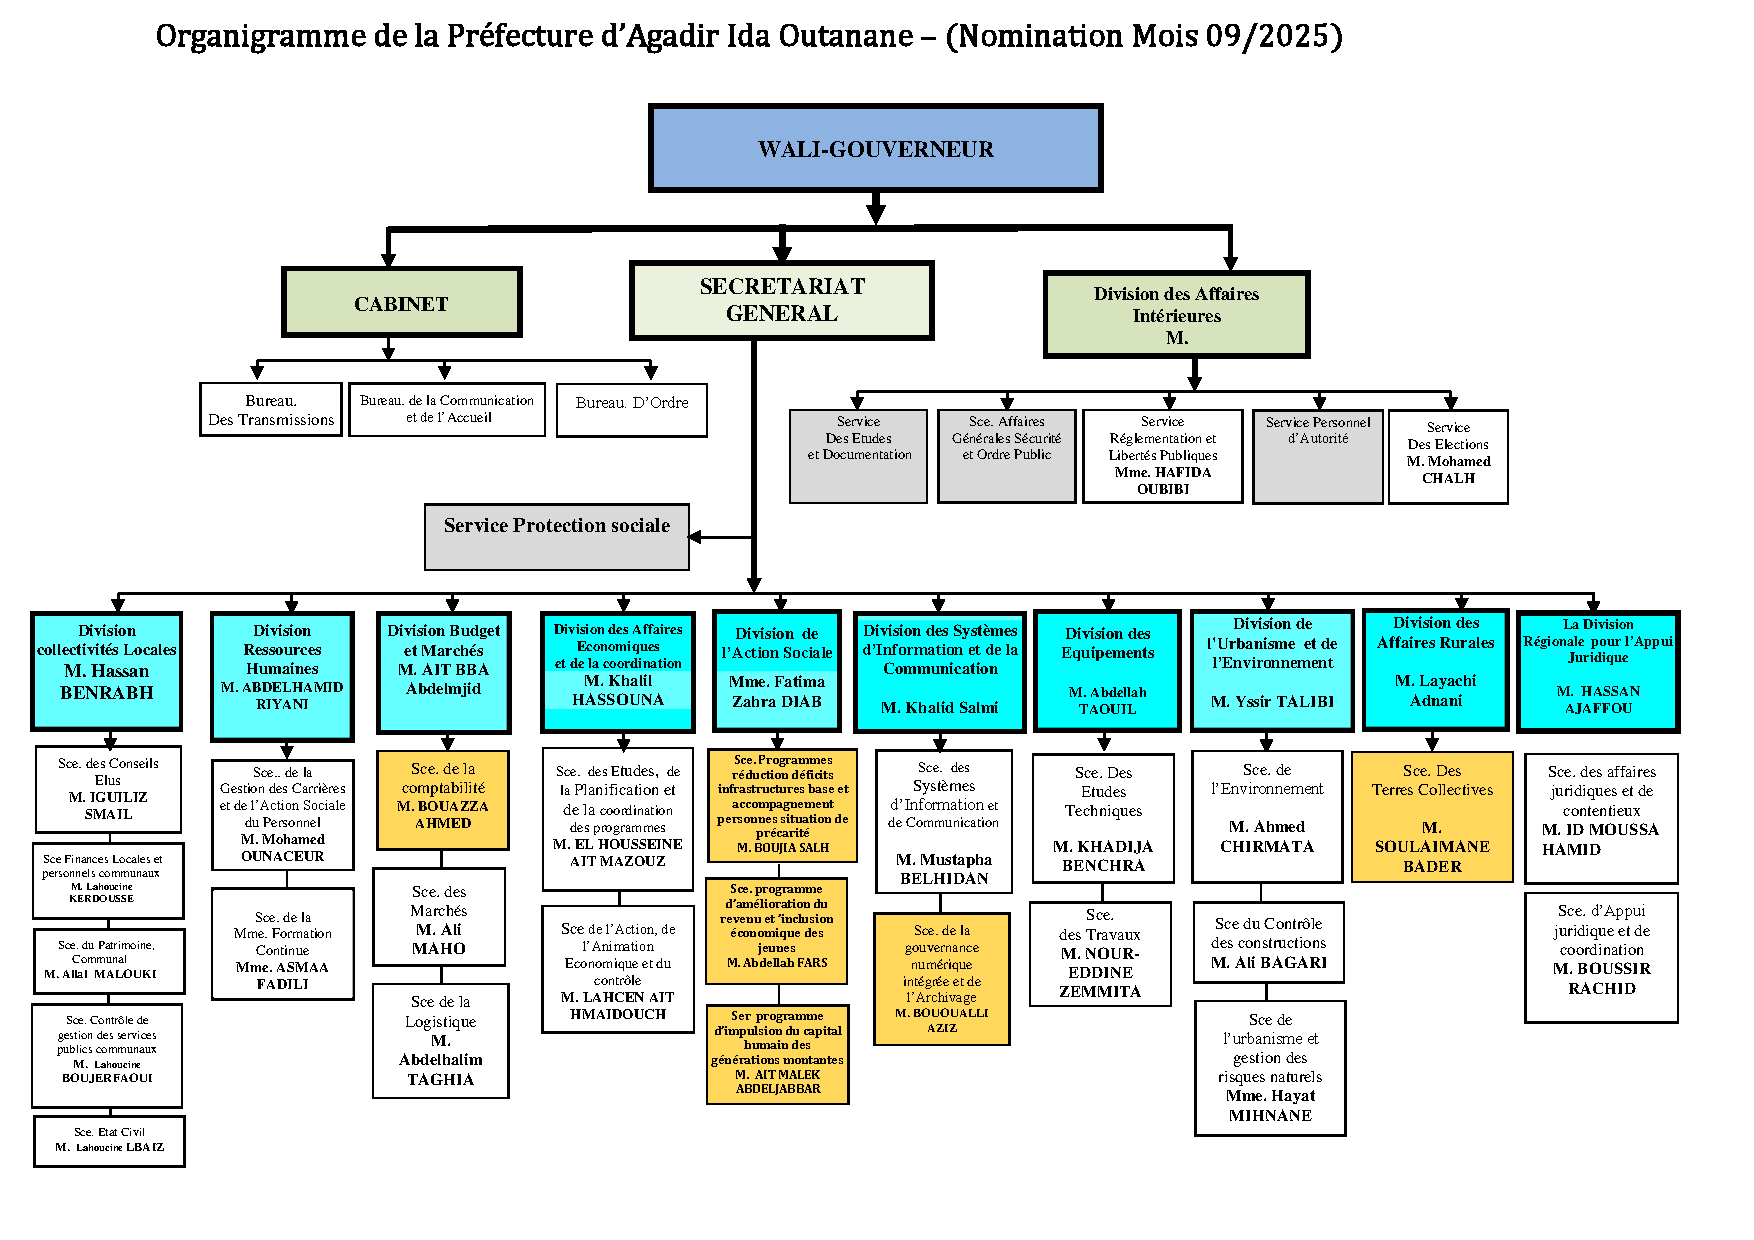
\includegraphics[width=0.8\textwidth, trim=1cm 1cm 1cm 1cm, clip]{../diagrams/organigramme.pdf}
    \caption{Organigramme de la Préfecture d'Agadir Ida Outanane}
    \label{fig:organigramme_wilaya}
\end{figure}

Cet organigramme met en évidence quatre niveaux structurels principaux~:

\begin{enumerate}
    \item Le \textbf{Wali-Gouverneur}, au sommet de la hiérarchie, qui dirige l'ensemble de la structure.
    \item Les \textbf{structures de direction et d'appui direct}, qui lui sont immédiatement rattachées. Elles sont composées du Cabinet, du Secrétariat Général et de la Division des Affaires Intérieures.
    \item Les \textbf{divisions opérationnelles et administratives}, majoritairement rattachées au Secrétariat Général. Ce pôle regroupe dix divisions métiers spécifiques :
    \begin{itemize}
        \item Division collectivités Locales
        \item Division Ressources Humaines
        \item Division Budget et Marchés
        \item Division des Affaires Economiques et de la coordination
        \item Division de l'Action Sociale
        \item Division des Systèmes d'Information et de la Communication
        \item Division des Equipements
        \item Division de l'Urbanisme et de l'Environnement
        \item Division des Affaires Rurales
        \item La Division Régionale pour l'Appui Juridique
    \end{itemize}
    \item Les \textbf{services (Sce.) et bureaux}, qui constituent l'échelon opérationnel de base. Chaque division, de même que le Cabinet ou la Division des Affaires Intérieures, se subdivise en plusieurs unités spécialisées (comme le Bureau d'Ordre, le Sce. des Marchés, le Sce. de l'Environnement, etc.) chargées de l'exécution concrète des tâches.
\end{enumerate}

% ==================== SECTION 1 ====================
\section{Contexte et objectifs}

L'organisation gère actuellement un ensemble de lignes de télécommunication (GSM, fixe, fax, ADSL, fibre optique) réparties sur le siège et ses annexes. Cette gestion est aujourd'hui effectuée de manière informelle, principalement par échanges d'emails, sans référentiel centralisé ni traçabilité structurée.

Le projet vise à automatiser et centraliser la gestion de ces flottes télécoms, en remplaçant le circuit actuel basé sur les échanges email par une application interne structurée, traçable, avec un circuit de validation hiérarchique et un reporting flexible.

\subsection{Objectif principal}
\begin{itemize}[leftmargin=*]
  \item Automatiser le processus de gestion des flottes télécoms (demande, validation hiérarchique, affectation, suivi, résiliation).
\end{itemize}

\subsection{Objectifs secondaires}
\begin{itemize}[leftmargin=*]
  \item Disposer d'un inventaire centralisé et fiable de l'ensemble des lignes (GSM, fixe/fax, ADSL, fibre).
  \item Assurer la traçabilité complète des demandes et décisions (qui a demandé quoi, qui a validé, quand).
  \item Permettre à chaque direction de suivre ses propres lignes via l'application, sans dépendre d'échanges email dispersés.
  \item Fournir un reporting flexible et filtrable (par direction, par type de flotte, par période, par statut).
\end{itemize}

% ==================== SECTION 2 ====================
\section{Périmètre du projet}

\subsection{Périmètre organisationnel}

\begin{itemize}[leftmargin=*]
  \item \textbf{Sites concernés} : Cluster du siège et ses annexes
  \item \textbf{Volume estimé} : Environ 600 utilisateurs
\end{itemize}

\subsection{Périmètre fonctionnel (types de flottes couvertes)}

\begin{center}
\begin{tabular}{L{4cm} L{11cm}}
\toprule
\rowcolor{tableheader}\textcolor{white}{\textbf{Élément}} & \textcolor{white}{\textbf{Détail}} \\
\midrule
GSM & Lignes mobiles (voix / data) attribuées aux agents \\
Fixe & Lignes téléphoniques fixes des postes de travail et services \\
Fax & Lignes ou postes dédiés à la transmission de fax (rattachés à la flotte fixe) \\
ADSL & Connexions internet ADSL des sites/annexes \\
Fibre optique & Connexions internet très haut débit des sites/annexes \\
\bottomrule
\end{tabular}
\end{center}

% ==================== SECTION 3 ====================
\section{Constat / problématique actuelle}

La gestion actuelle repose exclusivement sur des échanges par email entre les directions et les personnes en charge des télécoms. Cela entraîne plusieurs limites identifiées :

\begin{itemize}[leftmargin=*]
  \item Les échanges avec les opérateurs télécoms se font depuis des boîtes mail personnelles, sans rattachement systématique à un dossier ou une demande.
  \item Absence de référentiel centralisé de l'inventaire des lignes.
  \item Absence de traçabilité structurée des demandes et décisions.
  \item Absence de circuit de validation formalisé.
  \item Difficulté à produire un reporting consolidé et fiable.
\end{itemize}

\bigskip
\noindent\textit{Ce document d'expression de besoins pose le cadre, le contexte et les objectifs du projet. Les modalités fonctionnelles détaillées (acteurs, rôles, circuit de validation, cycle de vie des demandes) sont précisées dans le document Cahier des charges associé.}

\end{document}
